\documentclass[]{article}
\usepackage{float, graphicx, amsmath}
\setcounter{MaxMatrixCols}{20}
\setlength\parindent{0pt}
\begin{document}
\section{Linearization}
Letting  $\dot{x}=0$ we find a system of equations that holds for $v1^2 = v2^2 = v3^2 = v4^2 = g*m/(4*k*c_m) = 40.875$.
\\
The symbolic linearization around the equilibrium point $x^*$ becomes the following expression, we left out the sines and cosines which result in zero for the calculated equilibrium for readability: \\

\begin{align*}
\Delta \dot x &= 
\begin{pmatrix}
0 & 0 & 0 &1 &0 &0 &0 &0 &0 &0 &0 &0 \\
0 & 0 & 0 &0 &1 &0 &0 &0 &0 &0 &0 &0 \\
0 & 0 & 0 &0 &0 &1 &0 &0 &0 &0 &0 &0 \\
0 & 0 & 0 & -\frac{-k_d}{c} &0 &0 &0 & g &0 &0 &0 &0 \\
0 & 0 & 0 &0 &-\frac{-k_d}{c} &0 & -g&0 &0 &0 &0 &0 \\
0 & 0 & 0 &0 &0 &-\frac{k_d}{m} &0 &0 &0 &0 &0 &0 \\
0 & 0 & 0 &0 &0 &0 &0 &0 &0 &1 &0 &0 \\
0 & 0 & 0 &0 &0 &0 &0 &0 &0 &0 &1 &0 \\
0 & 0 & 0 &0 &0 &0 &0 &0 &0 &0 &0 &1 \\
0 & 0 & 0 &0 &0 &0 &0 &0 &0 &0 &0 &0 \\
0 & 0 & 0 &0 &0 &0 &0 &0 &0 &0 &d0 &0 \\
0 & 0 & 0 &0 &0 &0 &0 &0 &0 &0 &0 &0 \\
\end{pmatrix}\Delta x \\
& + \begin{pmatrix}
0 & 0 & 0 &0\\
0 & 0 & 0 &0\\
0 & 0 & 0 &0\\
0 & 0 & 0 &0\\
0 & 0 & 0 &0\\
\frac{k*c_m}{m} & \frac{k*c_m}{m} & \frac{k*c_m}{m}&\frac{k*c_m}{m}\\
0 & 0 & 0 &0\\
0 & 0 & 0 &0\\
0 & 0 & 0 &0\\
\frac{L*k*c_m}{I_{xx}} & 0 & -\frac{L*k*c_m}{I_{xx}} & 0 \\
0 & \frac{L*k*c_m}{I_{yy}} & 0 & - \frac{L*k*c_m}{I_{yy}} \\
\frac{b*c_m}{I_{zz}} & - \frac{b*c_m}{I_{zz}} & \frac{b*c_m}{I_{zz}} & -\frac{b*c_m}{I_{zz}} \\
\end{pmatrix} \Delta u \\
\end{align*}

\newpage
If we insert the numerical values of the symbols we get the following expression around the quilibrium:

\begin{align*}
\Delta \dot{x} &= 
\begin{pmatrix}
0 & 0 & 0 &1 &0 &0 &0 &0 &0 &0 &0 &0 \\
0 & 0 & 0 &0 &1 &0 &0 &0 &0 &0 &0 &0 \\
0 & 0 & 0 &0 &0 &1 &0 &0 &0 &0 &0 &0 \\
0 & 0 & 0 & -.5 &0 &0 &0 & 9.81 &0 &0 &0 &0 \\
0 & 0 & 0 &0 & -.5 &0 & -9.81&0 &0 &0 &0 &0 \\
0 & 0 & 0 &0 &0 &-.5 &0 &0 &0 &0 &0 &0 \\
0 & 0 & 0 &0 &0 &0 &0 &0 &0 &1 &0 &0 \\
0 & 0 & 0 &0 &0 &0 &0 &0 &0 &0 &1 &0 \\
0 & 0 & 0 &0 &0 &0 &0 &0 &0 &0 &0 &1 \\
0 & 0 & 0 &0 &0 &0 &0 &0 &0 &0 &0 &0 \\
0 & 0 & 0 &0 &0 &0 &0 &0 &0 &0 &0 &0 \\
0 & 0 & 0 &0 &0 &0 &0 &0 &0 &0 &0 &0 \\
\end{pmatrix}\Delta x \\
& + \begin{pmatrix}
0 & 0 & 0 &0\\
0 & 0 & 0 &0\\
0 & 0 & 0 &0\\
0 & 0 & 0 &0\\
0 & 0 & 0 &0\\
.06 & .06 & .06&.06\\
0 & 0 & 0 &0\\
0 & 0 & 0 &0\\
0 & 0 & 0 &0\\
1.5 & 0 & -1.5 & 0 \\
0 & 1.5 & 0 & - 1.5 \\
.1 & - .1 & .1 & -.1 \\
\end{pmatrix} \Delta u \\
\end{align*}

To verify our linearization we compared a simulation of it with the non-linear model. The linear model and the non-linear model gave the same result.The quadcopter flew straight up and was a little over 5 meter high after the simulated time of 5 seconds.

\begin{figure}[H]
\begin{minipage}{.5\textwidth}
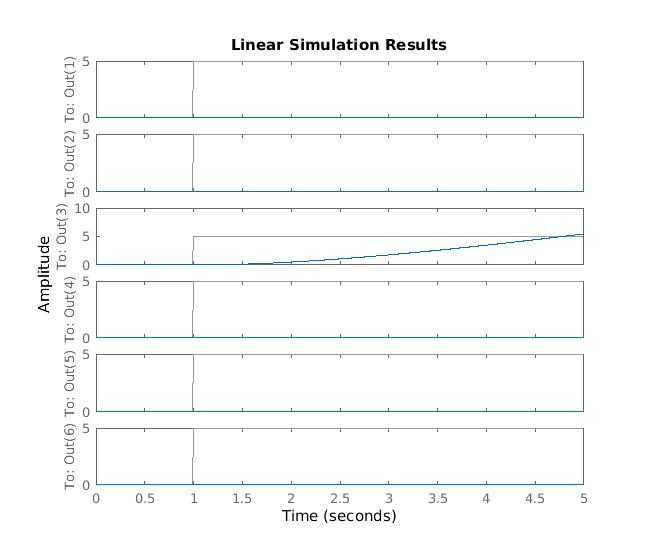
\includegraphics[width=\textwidth]{lsimresult.jpg}
\end{minipage}%
\begin{minipage}{.5\textwidth}
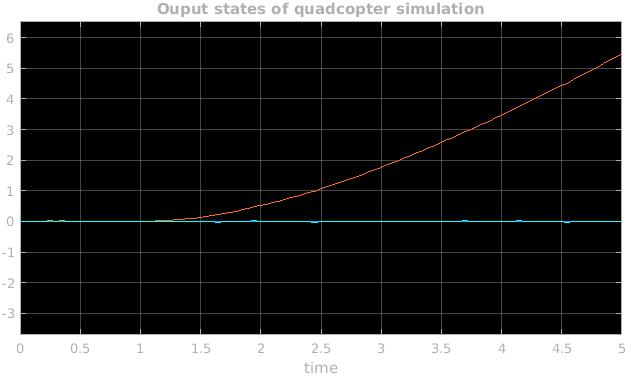
\includegraphics[width=\textwidth]{quadcoptersimresult.jpg}
\end{minipage}
\caption{Simulation of the linear model and the non-linear model with a step input.}
\end{figure}

\section{Discretization}
As a discretization rule the zero-order hold rule was used. The discretized matrices of the system are: \\
\begin{align*}
Ad &= \begin{pmatrix}
1	&0	&0&	0.049&	0	&0&	0&	0.012&	0	&0	&0.0003&	0 \\
0&	1&	0&	0&	0.049&	0&	-0.012&	0&	0&	-0.0003&	0&	0& \\
0	&0	&1&	0	&0	&0.049&	0	&0&	0&	0&	0&	0\\
0	&0	&0	&0.97&	0&	0&	0&	0.48&	0&	0&	0.012&	0 \\
0	&0	&0	&0	&0.97&	0&	-0.48&	0&	0&	-0.012&	0	&0& \\
0 &	0	&0	&0	&0	&.97&0	&0	&0	&0	&0	&0 \\
0 &	0	&0	&0	&0	&0	&1	&0	&0	&.05	&0	&0 \\
0 &	0	&0	&0	&0	&0	&0	&1	&0	&0	&.05	&0 \\
0 &	0	&0	&0	&0	&0	&0	&0	&1	&0	&0	&.05 \\
0 &	0	&0	&0	&0	&0	&0	&0	&0	&1	&0	&0 \\
0 &	0	&0	&0	&0	&0	&0	&0	&0	&0	&1	&0 \\
0 &	0	&0	&0	&0	&0	&0	&0	&0	&0	&0	&1 \\
\end{pmatrix} \\
\end{align*}
\begin{align*}
Bd &= \begin{pmatrix}
0 &	1.135e-05	&0	&-1.135e-05 \\
-1.135e-05	&0	&1.135e-05&	0 \\
7.41e-05 &	7.41e-05 &	7.41e-05&	7.41e-05 \\
0	&0.0005&	0&	-0.0005\\
-0.0005&	0&	0.0005&	0&\\
0.003&0.003&0.003&	0.003 \\
0.002 &	&0&	-0.002	&0 \\
0	&0.002 &	0	&-0.002 \\
0.0001&	-0.0001&	0.0001&	-0.0001 \\
0.075&&	0	-0.075&	0& \\
0	&0.075&	0&	-0.075& \\
0.005&	-0.005&	0.005&	-0.005 \\
\end{pmatrix} \\
Cd &= \begin{pmatrix}
1& 0& 0& 0.024& 0& 0& 0& -.00061& 0& 0& -1.5e^{-4}& 0 \\
0& 1& 0& 0& 0.024& 0& -.00061& 0& 0& -1.5e^{-4}& 0 & 0 \\
0& 0& 1& 0& 0& 0.024& 0& 0& 0& 0& 0& 0 \\
0& 0& 0& 0& 0& 0& 0& 0& 0& 0.025& 0& 0 \\
0& 0& 0& 0& 0& 0& 0& 0& 0& 0& 0.025& 0 \\
0& 0& 0& 0& 0& 0& 0& 0& 0& 0& 0& 0.025 \\
\end{pmatrix} \\
Dd &=\begin{pmatrix}
0& 5.67e^{-6}& 0& -5.67e^{-6}& \\
-5.67e^{-6}& 0& 5.67e^{-6}& 0& \\
3.7e^{-5}& 3.7e^{-5}& 3.7e^{-5}& 3.7e^{-5}& \\
9.35e^{-4}& 0& -9.35e^{-4}& 0& \\
0& 9.35e^{-4}& 0& -9.35e^{-4}& \\
6.25e^{-5}& 6.25e^{-5}& 6.25e^{-5}& 6.25e^{-5}& \\
\end{pmatrix}\\
\end{align*}

The system is completely controllable and observable. As all the states are controllable the system is stabilizable. As all the states are observable it is detectable. It is minimal as there are no uncontrollable and undetectable states. 

There are two transmission zeros in the system. Corresponding with the following states and inputs:

\begin{align*}
x_{zero1}=&\begin{pmatrix}
0 & \\ 
0 & \\ 
0 & \\ 
0 & \\ 
0 & \\ 
0 & \\ 
0 & \\ 
0 & \\ 
0 & \\ 
0 & \\ 
0 & \\ 
0.005 \\
\end{pmatrix}
&  u_{zero1} &= \begin{pmatrix}
.5 \\
-.5 \\
.5 \\
-.5 \\
\end{pmatrix} & x_{zero2} =&\begin{pmatrix}
0 & \\ 
0 & \\ 
0 & \\ 
0 & \\ 
0 & \\ 
0.003 & \\ 
0 & \\ 
0 & \\ 
0 & \\ 
0 & \\ 
0 & \\ 
0 \\
\end{pmatrix}
&  u_{zero2} &= \begin{pmatrix}
-.5 \\
-.5 \\
-.5 \\
-.5 \\
\end{pmatrix}
\end{align*}

\section{LQR/LQI control and robustness}
In the next three sections we will look at a lqr and a lqi controller for the quadcopter. We will then increase the mass of the quadcopter, which corresponds to adding a payload to it. We will see that while LQR is more optimal/faster if the physical model we deduced was exactly correct, it performs badly if some of the parameters were not estimated well. It is the other way around with integral contol. The controller is not the fastest or potimal, but  it is more robust and performs decently well with a payload. During the rest of the report the main design specification is to make the average time to reference points as short as possible while still reaching all the reference points. A second design criteria is that we aim for a trajectory which does not overshoot. A criteria that was not taken into account was the variance of the flight times between reference points. 

\subsection{LQR control}
To simulate the LQR control a scheme was created in simulink. The implemented scheme can be seen in the figure below. 

\begin{figure}[H]
\centering
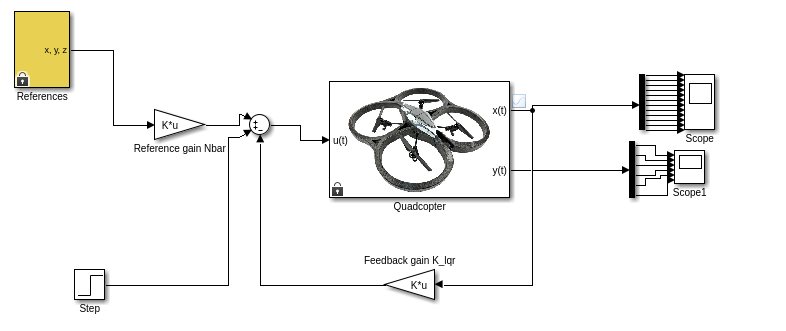
\includegraphics[width=.9\textwidth]{lqrscheme.png}
\caption{Simulink scheme of the quadcopter with lqr-control}
\end{figure}

Initially we set $Q = I$ and $R = I$, where $I$ denotes the identiy matrix of appropriate size. We get the following figures from the simulation. The trajectory in left picture of figure 2 shows that many of the checkpoints have not been reached. The output of the xyz-states show that this is mainly because the quadcopter moves too slowly to the z-coordinate of the reference points. The graph of the input signal, not shown here, also shows that the input signal is far from the clipping values, so there is much room for improvement.
\begin{figure}[H]
\begin{minipage}{.5\textwidth}
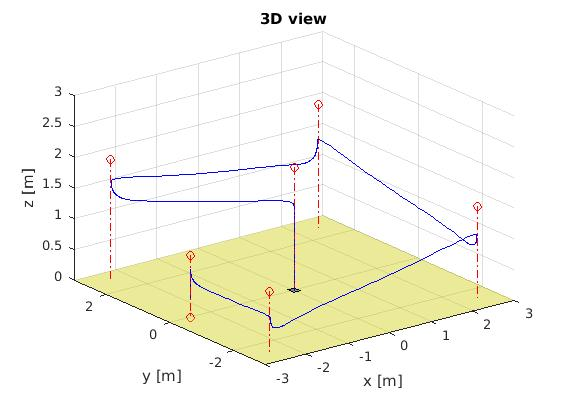
\includegraphics[width=\textwidth]{trajectory1.jpg}
\end{minipage}%
\begin{minipage}{.5\textwidth}
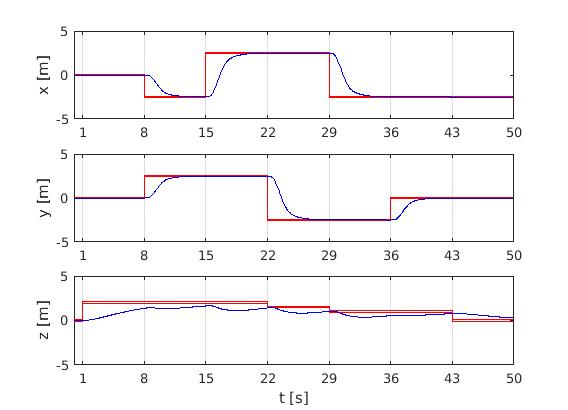
\includegraphics[width=\textwidth]{xyz1.jpg}
\end{minipage}
\caption{Tracjectory of the quadcopter and the xyz states for $Q = I$ and $R = I$}
\end{figure}

In a second try we increase all the diagonal values of $Q$ to 100. This should make the controller react stronger to changes in the reference signal over all states. It also makes sure the quadcopter returns to a neutral position more quickly after reaching a reference node. Figure 3 shows that with these settings the quadcopter reaches all the nodes. It does so in an average time of 4.179 seconds per node. 

\begin{figure}[H]
\begin{minipage}{.5\textwidth}
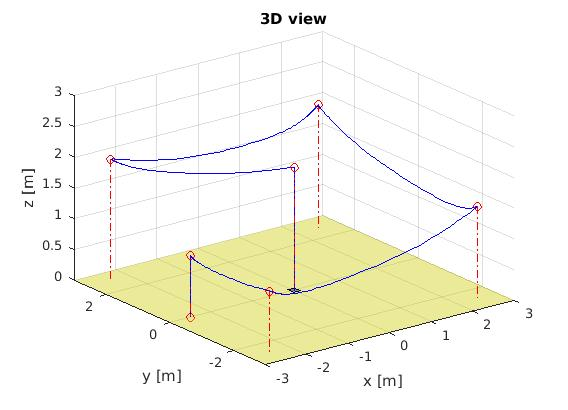
\includegraphics[width=\textwidth]{trajectory2.jpg}
\end{minipage}%
\begin{minipage}{.5\textwidth}
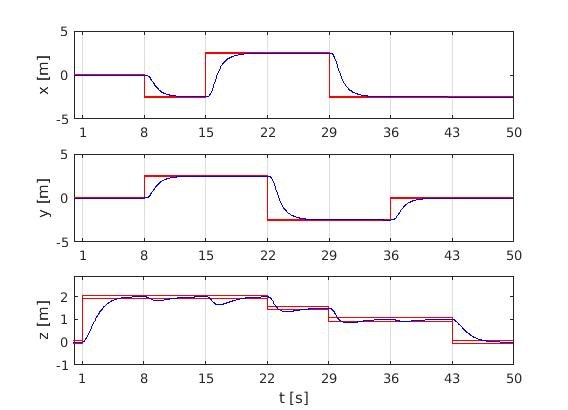
\includegraphics[width=\textwidth]{xyz2.jpg}
\end{minipage}
\caption{Tracjectory of the quadcopter and the xyz states for $Q = 100*I$ and $R = I$}
\end{figure}

Figure 3 shows that the quadcopter still does not react to the change in reference signals very fast. Therefore we set the first three diagonal values of $Q$ to 500. After doing so mainly the z-coordinate was lagging behind. This hints to the need of strongly increasing the value of Q which corresponds with reactions to the z-coordinate. A good average time of 1.327 was found for $Q(i,i) = 500$ for $i = 1,2$, $Q(3,3) = 50000$ and $Q(i,i) = 100$ for $i = 4,..,12$. The resulting trajectory is shown below in Figure 4. The average time to a node is 1.327 seconds.

\begin{figure}[H]
\begin{minipage}{.5\textwidth}
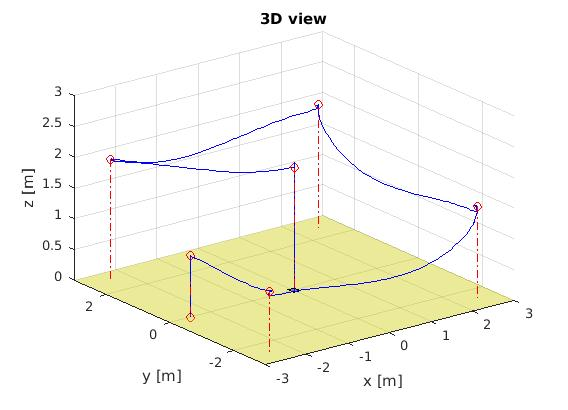
\includegraphics[width=\textwidth]{trajectory3.jpg}
\end{minipage}%
\begin{minipage}{.5\textwidth}
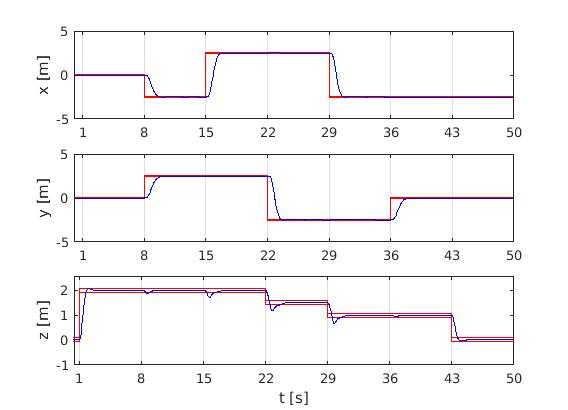
\includegraphics[width=\textwidth]{xyz3.jpg}
\end{minipage}
\caption{Tracjectory of the quadcopter and the xyz states for $Q(i,i) = 500$ for $i = 1,2$, $Q(3,3) = 50000$, $Q(i,i) = 100$ for $i = 4,..,12$ and $R = I$}
\end{figure}

\subsection{LQI control}
We now take a control which follows the reference input but we also add integral action. We extend the states with three states summing up the errors of the x,y and z coordinates over time. The created simulink model is shown in the figure below.

\begin{figure}[H]
\centering
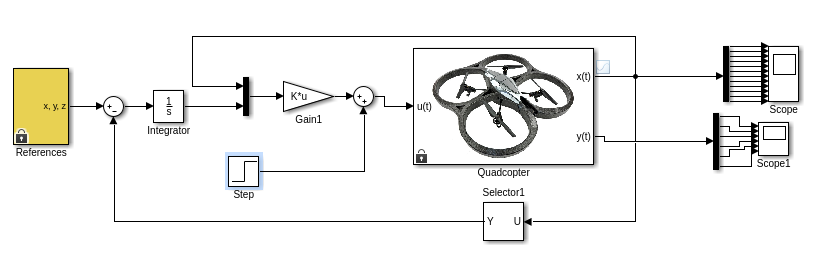
\includegraphics[width=.9\textwidth]{lqischeme.png}
\caption{Simulink scheme of the quadcopter with lqi-control}
\end{figure}

We again start with $Q = I$ and $R = I$ and get the simulated trajectory and output states shown in figure 6.   

\begin{figure}[H]
\begin{minipage}{.5\textwidth}
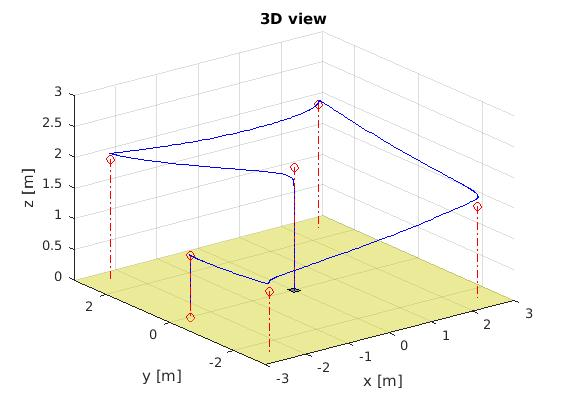
\includegraphics[width=\textwidth]{trajectoryi1.jpg}
\end{minipage}%
\begin{minipage}{.5\textwidth}
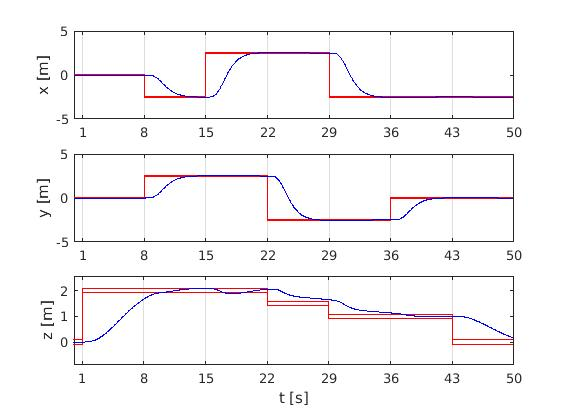
\includegraphics[width=\textwidth]{xyzi1.jpg}
\end{minipage}
\caption{Tracjectory of the quadcopter and the xyz states for $Q = I$ and $R = I$, integral control}
\end{figure}

As with LQR we notice that the checkpoints are not reached because dynamics of the closed loop are not fast enough. We increase the diagonal elements of Q to 200 and get the result shown in figure 7. All reference points were reached and the average time was 4.6 seconds. 

\begin{figure}[H]
\begin{minipage}{.5\textwidth}
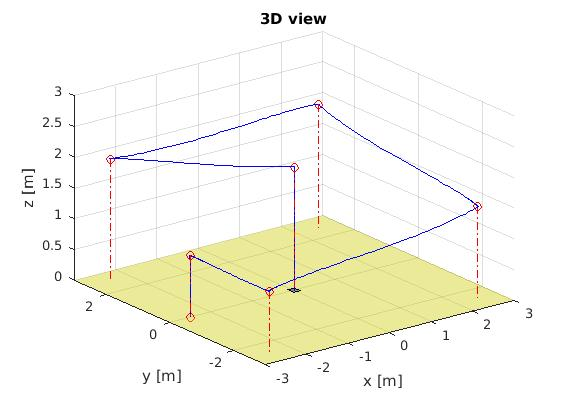
\includegraphics[width=\textwidth]{trajectoryi2.jpg}
\end{minipage}%
\begin{minipage}{.5\textwidth}
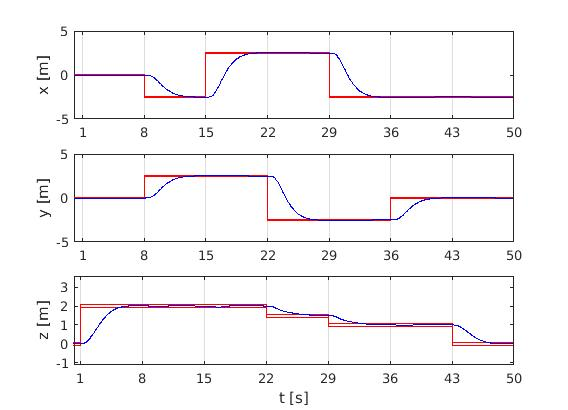
\includegraphics[width=\textwidth]{xyzi2.jpg}
\end{minipage}
\caption{Tracjectory of the quadcopter and the xyz states for $Q = 200*I$ and $R = I$, integral control}
\end{figure}

As with LQR control we modify $Q$ such that the quadcopter follows the references faster. To do this we change the values of Q related to the gain of the integral control. Setting $Q(i,i) = 10000$ for $i=13,14,15$ we get the result shown in figure 8. Average time to the reference points is 2.764 seconds.

\begin{figure}[H]
\begin{minipage}{.5\textwidth}
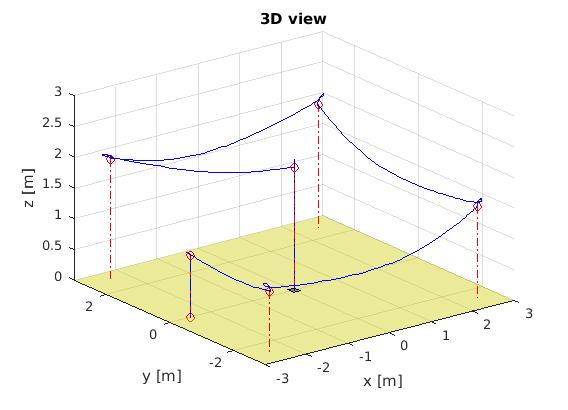
\includegraphics[width=\textwidth]{trajectoryi3.jpg}
\end{minipage}%
\begin{minipage}{.5\textwidth}
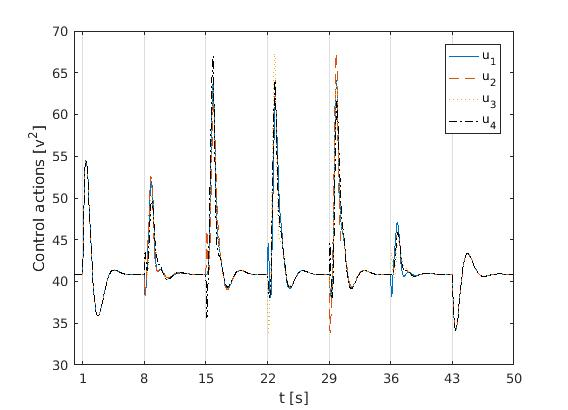
\includegraphics[width=\textwidth]{xyzi3.jpg}
\end{minipage}
\caption{Tracjectory of the quadcopter and the xyz states for $Q(i,i) = 10000*I$ for $i = 13,...,15$, $Q(i,i) = 200$ for $i = 1,...12$ and $R = I$, integral control}
\end{figure}

\subsection{Robusness, adding a payload}
If we add a payload of 0.1 kg to the model we get interesting results. Figure 8 shows the result for the LQR controller and the LQI controller. The $Q$ matrix for the lqr controller is $Q(i,i) = 200$ for $i = 1,2,4,...,12$ and $Q(3,3)=15000$ to make the system stable. Figure 9 nicely shows that the lqi controller is more robust to changes in the parameters. The simulation with lqr controller does not reach any of the reference points. The lqi controller does not perform as well as it did without the payload. The lqi scheme has an average delay of a second compared to the last situation situation, but it still reaches all the reference points.

\begin{figure}[H]
\begin{minipage}{.5\textwidth}
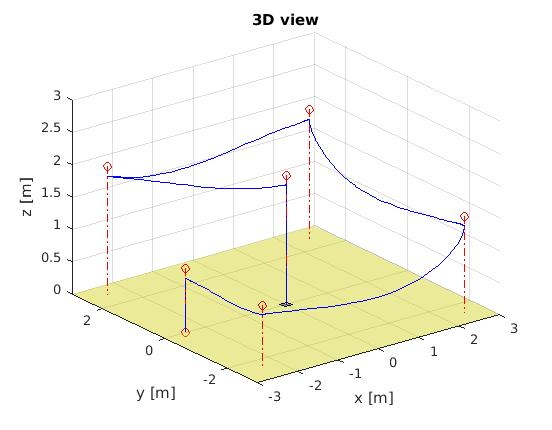
\includegraphics[width=\textwidth]{trajectorypayload.jpg}
\end{minipage}%
\begin{minipage}{.5\textwidth}
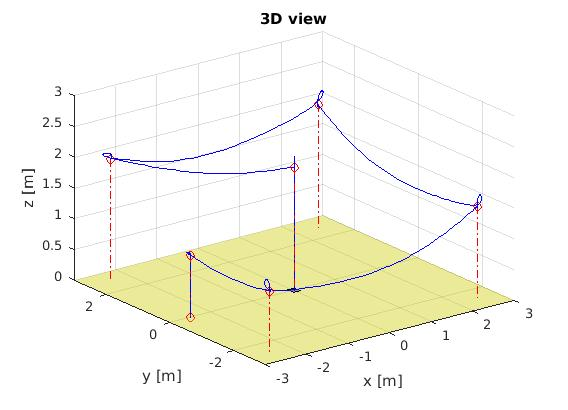
\includegraphics[width=\textwidth]{trajectorypayloadi.jpg}
\end{minipage}
\caption{Tracjectory of the quadcopter with payload. Left the lqr controller and right the lqi controller.}
\end{figure}

The fundamental difference between the controllers is that the lqi controller will reach reference points much better if the model is not exact, there is no steady sate error. The sum over the errors will at some point be strong enough to push the system to the required state, assuming that the input does not get saturated. In the LQR scheme it might be that error with respect to the reference point exactly balances with the inconsistency in the model, therefore a steady state error is created.

\section{LQG control}
In this section we discuss what happens if the full state vector is not available for feedback. Instead we will use the output and input of the system to estimate the current state. A scheme of the setup is shown in the figure below. 

\begin{figure}[H]
\centering
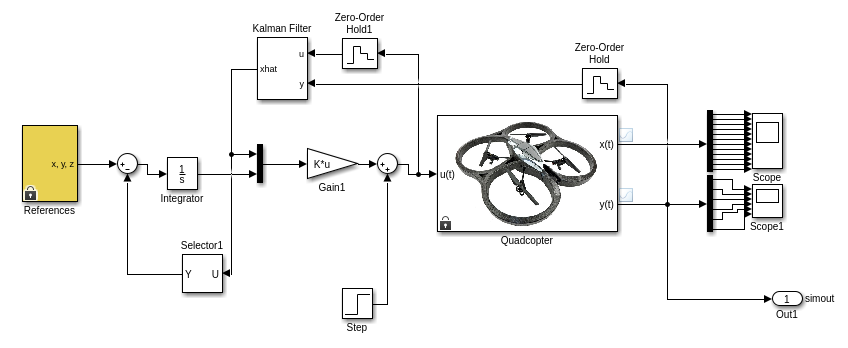
\includegraphics[width=.9\textwidth]{kalscheme.png}
\caption{Simulink scheme of the quadcopter with lqi-control and kalman filter}
\end{figure}

The choice of the matrix for the process noise is a simplification of the piecewise white noise model. A motivation for this simplification is described on page 243 of the book "Kalman and Bayesian filter in Python" by Roger R Labbe. In the text it explains why the noise can be approximated by only adding process noise to the faster states of the system. However, the magnitude of the variance is still not taken into account. If we overestimate the processnoise the system is too slow, if we underestimate the noise, the filter is overly confident. We found that a variance of 0.01 gives good results. 
\\\\
For this new scheme we again start with a simulation where $Q=I$ and $R=I$. This gives us the results shown below. The quadcopter does not reach the reference points as can be seen in the left figure. Both figures show that this is mainly because the z-coordinate lags behind too much.

\begin{figure}[H]
\begin{minipage}{.5\textwidth}
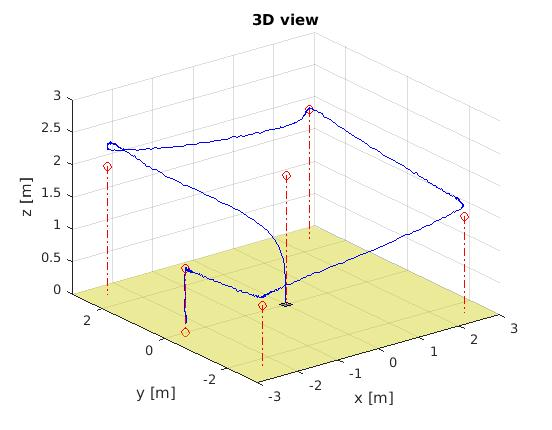
\includegraphics[width=\textwidth]{kaltraj1.jpg}
\end{minipage}%
\begin{minipage}{.5\textwidth}
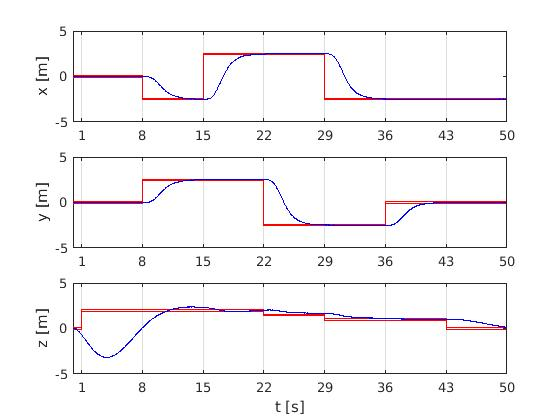
\includegraphics[width=\textwidth]{kalstate1.jpg}
\end{minipage}
\caption{Trajectory and xyz-states of the quadcopter simulation using a kalman-filter and lqi-scheme.}
\end{figure}

To correct this we increase the reaction of the controller to errors with respect to the z-reference points. We also increase the terms corresponding to faster reactions to the summed error terms, increasing the integral control. This leads to much better behavior. Average time to a reference point is 2.621.

\begin{figure}[H]
\begin{minipage}{.5\textwidth}
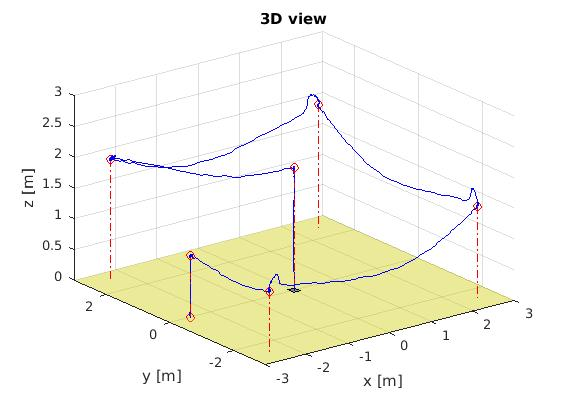
\includegraphics[width=\textwidth]{kaltraj2.jpg}
\end{minipage}%
\begin{minipage}{.5\textwidth}
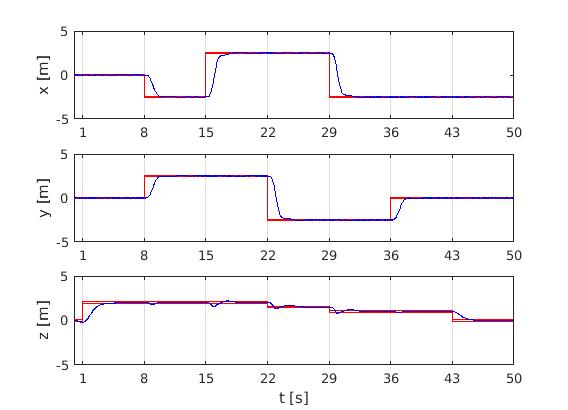
\includegraphics[width=\textwidth]{kalstate2.jpg}
\end{minipage}
\caption{Trajectory and xyz-states of the quadcopter simulation using a kalman-filter and lqi-scheme, Q(i,i)  = 200 for i = 1,2, Q(3,3) = 5000, Q(j,j) = 200 for j = 1,...12, Q(k,k) = 11000 for k = 13,14,15. }
\end{figure}

If we add a payload of 0.1 kg and we keep using the last settings we get good performance. The quadcopter experiences an average delay of only 0.186 seconds per reference point. The trajectory of the quadcopter and its xyz-states over the course of the simulation are displayed below. 

\begin{figure}[H]
\begin{minipage}{.5\textwidth}
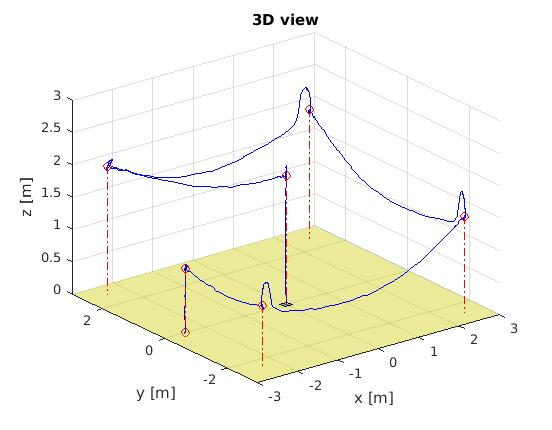
\includegraphics[width=\textwidth]{kaltraj2pay.jpg}
\end{minipage}%
\begin{minipage}{.5\textwidth}
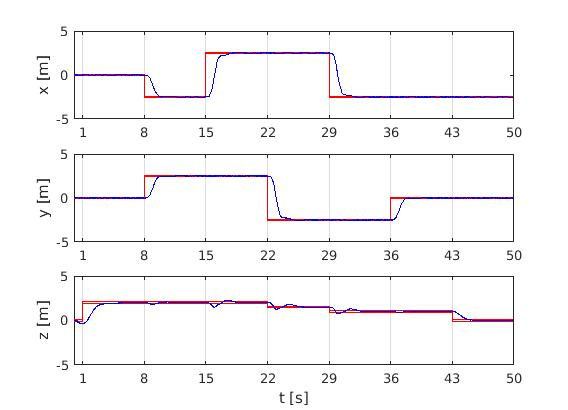
\includegraphics[width=\textwidth]{kalstate2pay.jpg}
\end{minipage}
\caption{Trajectory and xyz-states of the quadcopter with payload simulation using a kalman-filter and lqi-scheme, Q(i,i)  = 200 for i = 1,2, Q(3,3) = 5000, Q(j,j) = 200 for j = 1,...12, Q(k,k) = 11000 for k = 13,14,15. Payload is 0.1 kg.}
\end{figure}

\section{Conclusions}
To compare the different schemes we have a look at the following table. It presents the average flight time to the reference points for all three schemes with and without payload. The lqr scheme is clearly the fastest for the situation without payload, but fails when the model is not correct. In the other situation the lqi scheme without kalman filter is faster than the situation with kalman fitler. This is as expected, as the states we use for feedback are estimated and therefore less correct. Interestingly there are settings for Q and R where the lqi-scheme with payload is faster than without the payload as can be seen in the table below. The average flight times for lqi and kalman with payload were achieved with Q(i,i)  = 1500 for i = 1,2, Q(3,3) = 3000, Q(j,j) = 1500 for j = 1,...12, Q(k,k) = 40000 for k = 13,14,15. 

\begin{figure}[H]
\centering
\begin{tabular}{|c|c|c|}
\hline
& wihout payload & with payload \\
\hline
lqr-scheme &  1.326s  & n.a.   \\
lqi-scheme &  1.907s	&  1.886s \\
lqi-kalman scheme & 2.386s	 & 2.536s \\
\hline
\end{tabular}
\end{figure}

We also have a look at the input signals for the schemes without payload, these are displayed below. The input signal of the kalman-filter is much more violent. This might be as expected as we have to estimate the states using noisy signals. The input signals for the lqr and lqi schemes are smoother. 

\begin{figure}[H]
\begin{minipage}{.3\textwidth}
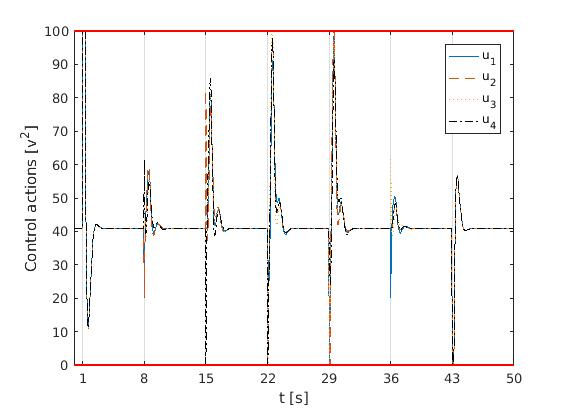
\includegraphics[width=\textwidth]{lqrinput.jpg}
\end{minipage}%
\begin{minipage}{.3\textwidth}
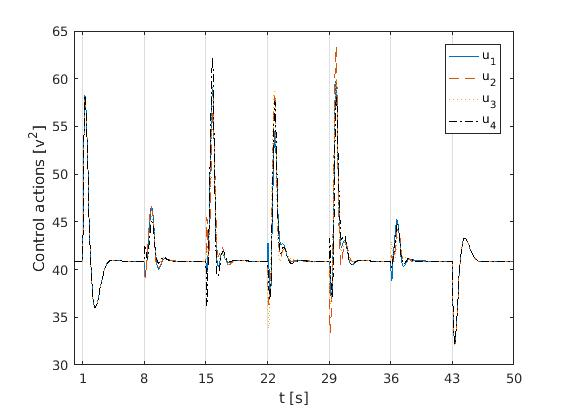
\includegraphics[width=\textwidth]{lqiinput.jpg}
\end{minipage}
\begin{minipage}{.3\textwidth}
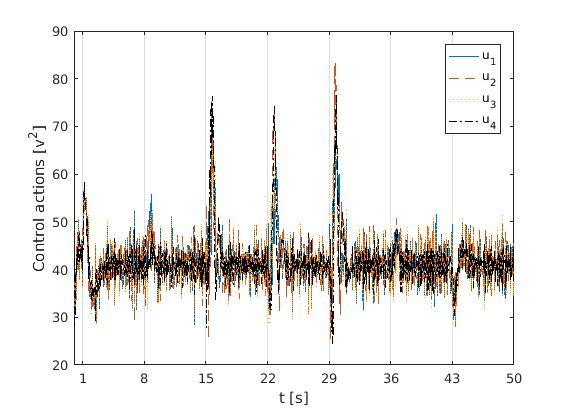
\includegraphics[width=\textwidth]{kalinput.jpg}
\end{minipage}
\caption{Input signals for a simulation of different schemes corresponding with the resulting flight times in the table above. From left to right the input for the lqr, lqi and lqi/kalman scheme}
\end{figure}

\end{document}